To determine the behavior of a folded optical spring, we can compare it to the standard optical spring derivation \cite{Perreca14}.

We begin with a folded cavity with three mirrors, shown in fig. \ref{f:angularLayout}. The incoming field is E. The average round-trip path length is $L = 4L_0$. We consider microscopic harmonic changes in cavity length $d_n$ corresponding to mirror positions at specific times $d(t)$ moving mirrors M3 and M4 for $n$ odd and even, respectively. The light travel time in one `arm' is $\tau = \frac{L_0}{c}$.

\begin{figure}[p]
\vspace{5pt}
\begin{center}
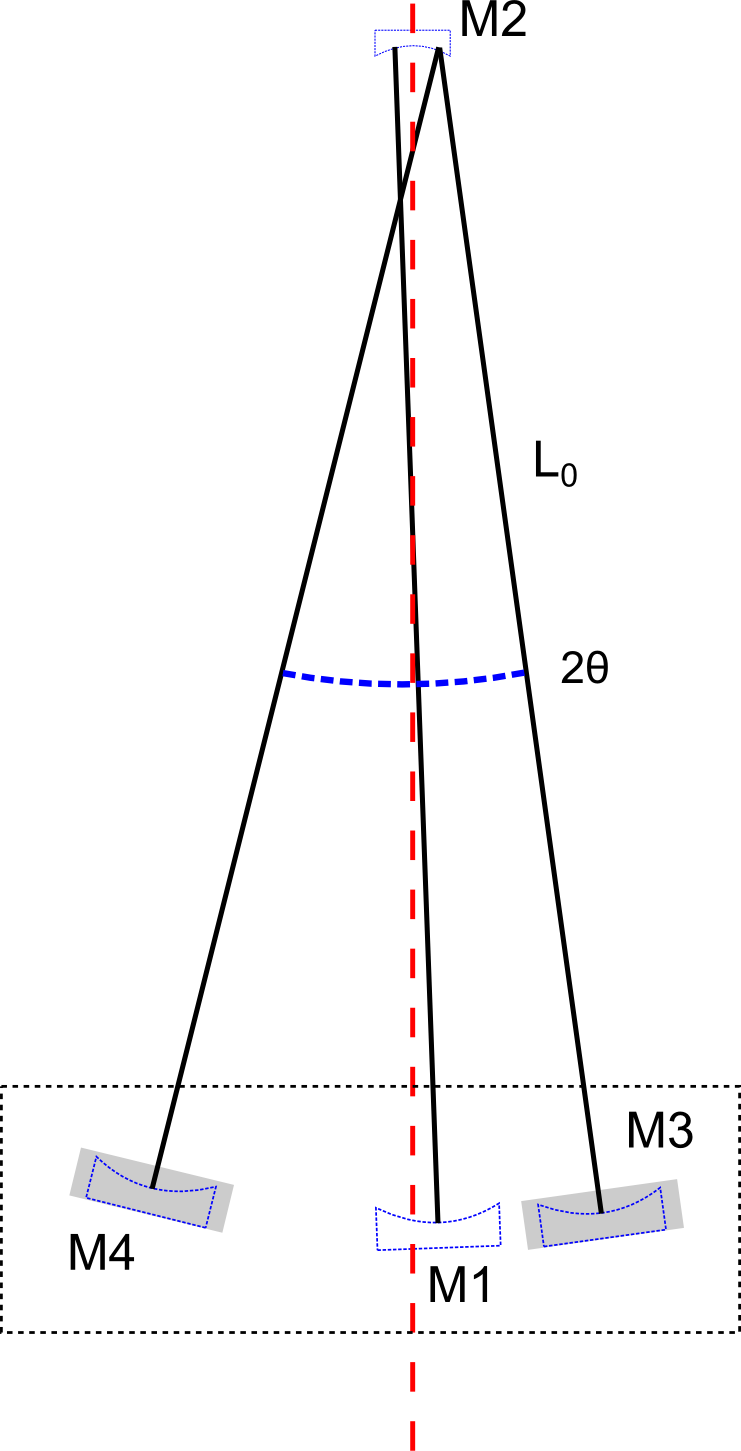
\includegraphics[width=.5\textwidth]{figures/angular/angularLayout}
\end{center}
\caption[Folded cavity layout]{%
\label{f:angularLayout}
Layout of the angular trap cavity. Light enters through mirrors M1 and M3.
}
\end{figure}

We can write the round trip path length including the noise as

\begin{eqnarray}
L_1&=&2(2L_0+d_1+d_2)\\
L_2&=&2(4L_0+d_1+d_2+d_3+d_4)\nonumber\\
L_3&=&2(3L_0+d_1+d_2+d_3+d_4+d_5+d_6)\,\, \nonumber\\
...\nonumber
\label{e:L}
\end{eqnarray}



\begin{eqnarray}
\label{e:dn}
d(t) &=& x_0 e^{i\Omega t}\nonumber\\
d_n &=& d(t-[(2n-1)\tau + \alpha_n ]) \quad \mbox{and}\\
\label{e:an}
\alpha_n &=& 2\sum\limits_{l=1}^{n-1}\frac{d_l}{c}-\frac{d_n}{c}
\end{eqnarray}

We define a phase propagation $Y=e^{-i\Omega 2\tau}$ and cavity round trip propagation $X=(r_1r_2)^2 e^{\frac{-i2\pi L}{\lambda}}$. Neglecting the $\alpha_n$ terms, which are quadratic in $d$,

\begin{eqnarray}
\label{e:dnY}
d_n &=& Y^{2(n-1)}d_1\\
d_{n+1} &=& Y^2d_n\nonumber
\end{eqnarray}

following Antonio,

\begin{eqnarray}
\label{e:Etot}
E_{tot} = \frac{t_1 E}{1-X}\left[ 1- \frac{4i\pi d_1}{\lambda}\frac{X(1+Y^2)}{1-Y^2X}\right]\nonumber\\
E_{tot} = \frac{t_1 E}{1-X}\left[ 1- \frac{4i\pi}{\lambda}\left(\frac{ d_1(1+Y^2)}{1-Y^2X}+\frac{ \overline{d_1}(1+\overline{Y}^2)}{1-\overline{Y}^2X}\right)\right]
\end{eqnarray}

$d_1 = xY$ so we get the power 

\begin{eqnarray}
\label{e:P}
%P&=&E_{tot}\cdot \overline{E}_{tot}=P_0 t^2[ \frac{1}{(1-X)(1-\overline{X})}\nonumber\\  
%&-&\frac{ikX xY}{(1-\overline{X})(1-X)(1-Y^2 X)} -
%\frac{ikX \bar{x}\overline{Y}}{(1-\overline{X})(1-X)(1-\overline{Y}^2 X)}\nonumber \\
%&+&\frac{ik\overline{X} \bar{x}\overline{Y} } {(1-\overline{X})(1-X)(1-\overline{Y}^2 \overline{X})}+ 
%\frac{ik\overline{X} xY}{(1-\overline{X})(1-X)(1-Y^2 \overline{X})}]  \nonumber \\
P &=&-P_0t^2 \left[ \frac{ikY}{(1-\overline{X})(1-X)} \left( \frac{X(1+Y^2)}{1-Y^2 X}-\frac{\overline{X}(1+\overline{Y}^2)}{1-Y^2\overline{X}} \right) x + cc \right]?
\end{eqnarray}


